

\author[Jannis Klingler]{Nix}


\beamertemplatenavigationsymbolsempty{}

\logo{
\includegraphics[height=1cm]{Bilder/logo}}



\section{Variational Autoencoder}

\begin{frame}
	\frametitle{Beispiel \emph{time series}}
	\begin{figure}[!htbp]
		
\includegraphics[scale=0.25]{Bilder/rotatingMNIST}\\
		Beispiel einer \emph{time series} bestehend aus \\10 Bildern des Datensatzes rotatingMNIST
	\end{figure}
\end{frame}

\begin{frame}
	\frametitle{Modellannahmen}
	Gegeben:
	\begin{itemize}
		\item Datensatz $\textbf{X} = \lbrace\x \rbrace_{i=1}^{N} \subset \R^{D\times N}$
		\item Datenpunkte $\x\sim p(\x)$ (u.i.v. Realisierungen einer hochdimensionalen Zufallsvariable)
	\end{itemize}
\end{frame}

\begin{frame}
	\frametitle{Latente Variablen Modell}
	Suchen:
	\begin{itemize}
		\item Verteilung der Datenpunkte $\x$
		\item Eine niedrigdimensionale Darstellung der Daten, die den Prozess, der die Daten erzeugt, möglichst gut modelliert
		\item Führen dazu \emph{Latente Variablen} $\z$, die auf dem \emph{latenten Raum} $\mathcal{Z} = \R^d$ mit $d\ll D$ definiert sind, ein.
	\end{itemize}
\end{frame}

\begin{frame}
	\frametitle{Latente Variablen Modell}
	Das \emph{Latente Variablen Modell} besteht nun aus den Verteilungen:
	\begin{itemize}
		\item Verteilung der Daten $p(\x)$
		\item Posteriorverteilung $p(\z|\x)$ \quad(später Encoder)
		\item Priorverteilung $p(\z)$
		\item Generatives Modell $p(\x|\z)$ \quad(später Decoder)
	\end{itemize}
\end{frame}

\begin{frame}
	\frametitle{Latente Variablen Modell}
	Sind interessiert an der Verteilung
	\[p(\x)= \int_{\z} p(\x,\z) \mathrm{d}\textbf{z} = \int_{\z} p(\x|\z)p(\z) \mathrm{d}\z.\]
	\textbf{Problem:} Dieses Integral kann aufgrund der hohen Dimension des Raumes $\mathcal{X}$ und der Komplexität des Modells 
	nicht berechnet und auch nicht sinnvoll approximiert werden. \\ \ 
	\\
	Mit dem Satz von Bayes gilt dies auch für die Verteilung
	\[p(\z|\x)= \frac{p(\x|\z)p(\z)}{p(\x)}.\]
\end{frame}

\begin{frame}
	\frametitle{Implementierung}
		\begin{itemize}
		\item Führen nun das Inferenzmodell $q_{\boldsymbol\phi}(\z|\x)$ ein und suchen die Parameter $\boldsymbol\phi^{*}$ für die $q_{\boldsymbol\phi^{*}}(\z|\x) \approx p_{\boldsymbol\theta}(\z|\x)$ gilt 
		\item In einem Variational Autoencoder werden die Verteilungen $q_{\boldsymbol\phi}(\z|\x)$ und $p_{\boldsymbol\theta}(\x|\z)$ durch neuronale Netze dargestellt und approximiert
		\item Können dann die Verteilung von $p(\z)$ festlegen (häufig $\mathcal{N}(0,\textbf{I})$)
	\end{itemize}
\end{frame}

\begin{frame}
	\frametitle{Schematische Darstellung der VAE-Architektur}
	\begin{figure}[htbp!]
		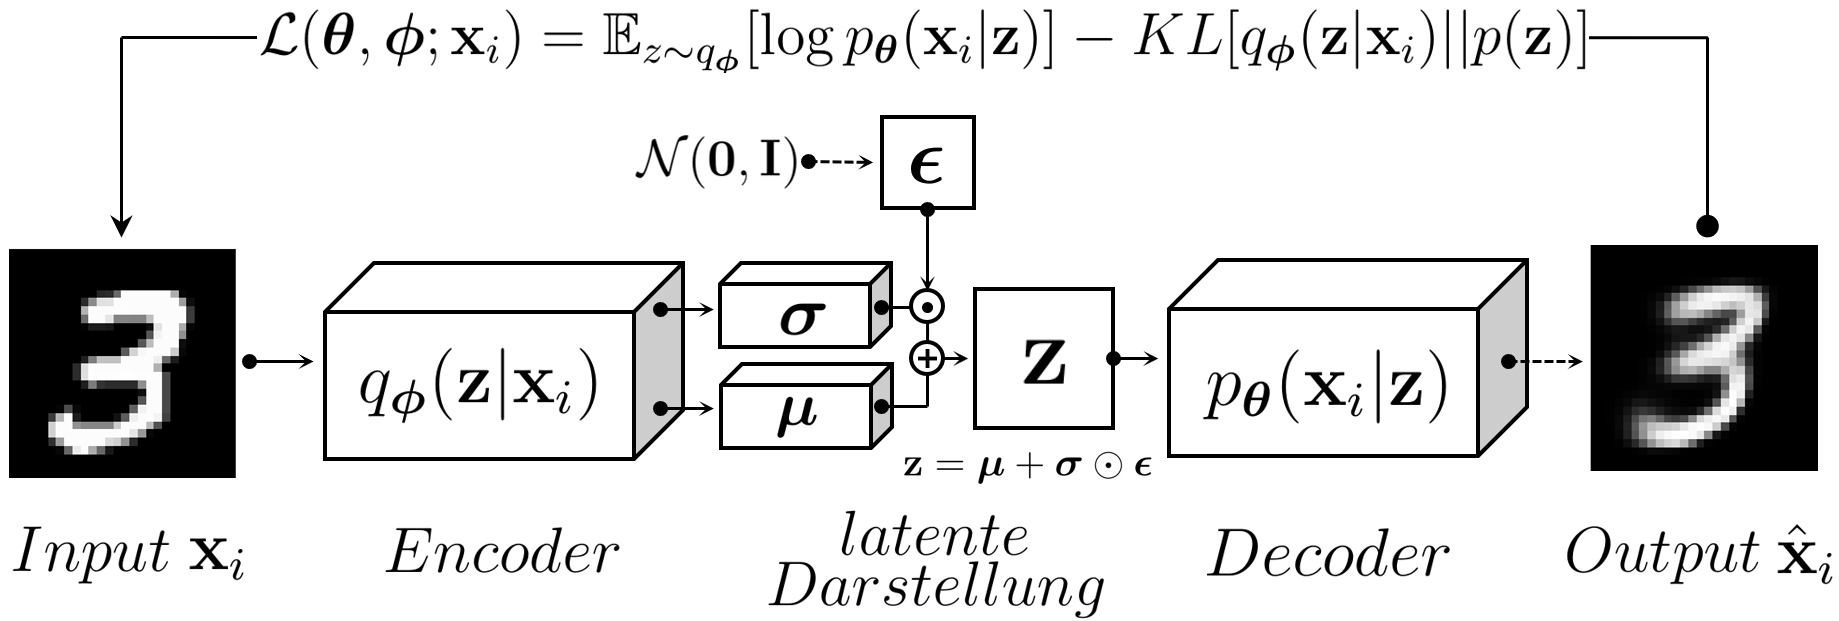
\includegraphics[scale=0.27]{Bilder/VAE-Modell.PNG}
	\end{figure}
\end{frame}